\chapter{Descrição das bases de Dados utilizadas}

\section{Empresa de Bebidas} \label{sec:AppBDAmbev}

\singlespacing
\begin{table}[ht]
    \caption{Principais variáveis observadas na Base de Dados.}
    \resizebox{\textwidth}{!}{\begin{tabular}{|ccc|}
    \hline
    \cellcolor[HTML]{BFBFBF}\textbf{Variável} & \cellcolor[HTML]{BFBFBF}\textbf{Descrição} & \cellcolor[HTML]{BFBFBF}\textbf{Intervalo}\\
    Data        & Dia em que a rota foi realizada.      & 03/01/2015 a 30/05/2015\\
    Mapa        & Identificador de rota de entregas.    & 4620 códigos únicos\\
    Placa       & Identificador veículo da rota.        & 42 distintos\\
    Id. Cliente & Identificador de cliente.             & 4554 distintos (916xxxxx)\\
    Seq Real    & Ordem real da entrega.                & (vazio); 1 a 43\\
    Seq Plan    & Ordem planejada da entrega            & 1 a 43\\
    Inicio Rota & Horário de início da rota.            & N.R.; 05:09:25 a 19:51:05\\
    Saída CDD   & Horário de saída do CDD.              & 06:06:00 a 20:05:00\\
    Chegada ao PDE & Horário de chegada ao PDE.         & 06:50:26 a 23:49:01\\
    Inicio Entrega & Horário de início da entrega.      & 06:50:26 a 23:49:01\\
    Fim Entrega    & Horário finalização da entrega.    & 00:05:21 a 23:42:02\\
    Fim Rota    & Horário finalização da rota        & 07:35:41 a 00:00:24\\
    Entrada CDD    & Horário retorno ao CD.            & 06:58:21 a 01:32:00\\
    Caixas carregadas & Volume de caixas a serem entregues. & 0 a 589,75\\
    Caixas devolvidas & Volume de caixas devolvidas.    & 0 a 416,15\\
    Repasse     & Qtde. de repasses em um PDE numa mesma rota. & 0 a 10\\
    Tempo de entrega        & Tempo total da entrega (descarga + espera).    & (vazio); 00:00:00 a  09:32:46 \\
    Tempo Descarga          & Tempo de descarga da entrega. & 00:00:00 a 01:57:57\\
    Tempo Espera            & Tempo de espera da entrega. & 00:00:00 a 08:09:50\\
    Tempo total de rota     & Tempo total de rota.        & (vazio); 00:00:00 a 71:10:36\\
    Tempo Deslocamento  & Tempo efetivo de deslocamento do veículo. & 00:00:00 a 22:54:19\\
    Lat. Cliente        & Latitude do cliente.  & (vazio); -23,xxxxxxxx\\
    Lon. Cliente        & Longitude do cliente. & (vazio); -4x,xxxxxxxx\\
    Distância Prev.     & Distância planejada (km).  & (vazio); 0,08 a 36,29         \\
    Distância Perc. Apontamento & Distância real percorrida (km). & (vazio); 0,002 a 12.355,18 \\ \hline
    \end{tabular}}
    \label{tab:Variaveis_BD}
    \caption*{Fonte: Produzido pelos autores Fernandes \& Alves}
\end{table}
\onehalfspacing

\section{Amazon} \label{sec:appDBAmazon}

% A seguir, são apresentadas as principais fontes de informações disponíveis na base de dados utilizada.
A base de dados pode ser facilmente copiada do servidor \textit{Amazon Simple Storage Service} (s3) (\citeauthoronline{aws_s3}, \citeyear{aws_s3}), sem a necessidade de realizar login ou cadastro.
%

O diretório disponível está representado abaixo:

\begin{lstlisting}
\---almrrc2021
    |   License.txt
    |   Readme.txt
    |
    \---almrrc2021-data-training
        +---...
        |
        +---model_build_inputs
        |       new_package_data.json
        |       new_route_data.json
        |       new_travel_times.json
        |       readme.md
        |       
        +---...
\end{lstlisting}

Do arquivo \textit{new\_package\_data.json} é possível obter informações relativas aos pacotes de cada entrega, como por exemplo suas dimensões e código identificador.
%
Cada conjunto de pacotes é associado a uma das \textit{stops} presentes no arquivo \textit{new\_route\_data.json}, o qual carrega os detalhes de coordenadas geográficas e disponibilidade horária de entrega de cada cliente observado na rota, bem como os CDs associados.
%
O aquivo \textit{new\_actual\_sequences.json} é o indexador que permite organizar as paradas de cada rota de acordo com a sequência real observada no dia da entrega.
%
O arquivo \textit{new\_travel\_times.json}, por sua vez, traz consigo uma matriz de distâncias para todos os pontos da base em estudo.
%
Contudo, esta matriz é preenchida somente com valores de tempo de percurso entre os distintos pontos, ignorando totalmente a informação de distância percorrida associada aos percursos.
%
Apesar de não se tratar de uma limitação, tal fato implica em uma dificuldade a mais para o trabalho dos autores, que, dados os objetivos da pesquisa, tiveram que adotar outros mecanismos para cálculo dessas determinadas distâncias. Por fim, o arquivo \textit{read.md} simplesmente contém uma breve descrição dos arquivos presentes no diretório.

\chapter{Informações Geográficas}\label{sec:AppGIS}

\section{Guarulhos, SP - Brasil}

A Tabela \ref{tab:dados-espaco-gru} apresenta os bairros disponíveis na fonte de dados de informação geoespacial utilizada para a cidade de Guarulhos durante a realização do primeiro estudo de caso.

% \begin{spacing}{1}
\begin{table}[H]
    \caption{Bairros disponíveis na fonte de dados de informações espaciais.}
    \label{tab:dados-espaco-gru}
    \centering
    \resizebox{\textwidth}{!}{\begin{tabular}{|cccc|cccc|}
        \hline
        \rowcolor[HTML]{BFBFBF} 
        \multicolumn{1}{|c|}{\cellcolor[HTML]{BFBFBF}\textbf{index}} & \multicolumn{1}{c|}{\cellcolor[HTML]{BFBFBF}\textbf{Nome do Bairro}} & \multicolumn{1}{c|}{\cellcolor[HTML]{BFBFBF}\textbf{landuse}} & \textbf{area (km²)} & \multicolumn{1}{c|}{\cellcolor[HTML]{BFBFBF}\textbf{index}} & \multicolumn{1}{c|}{\cellcolor[HTML]{BFBFBF}\textbf{Nome do Bairro}} & \multicolumn{1}{c|}{\cellcolor[HTML]{BFBFBF}\textbf{landuse}} & \textbf{area (km²)} \\ \hline
        0 & Cabuço de Cima &  & 24,5 & 19 & Gopoúva & res. & 2,1 \\
        1 & Cabuçu &  & 19,3 & 20 & Jardim Vila Galvão & res. & 1,3 \\
        2 & Mato das Cobras &  & 10,2 & 21 & Itapegica & res. & 3,2 \\
        3 & Morro Grande &  & 56,2 & 22 & Monte Carmelo & res. & 0,5 \\
        4 & Sadokim &  & 3,0 & 23 & Morros & res. & 3,7 \\
        5 & Bonsucesso &  & 20,9 & 24 & Ponte Grande &  & 3,5 \\
        6 & Jardim Pres. Dutra & res. & 4,4 & 25 & Porto da Igreja &  & 3,4 \\
        7 & Bom Clima & res. & 1,0 & 26 & Picanço & res. & 3,0 \\
        8 & Lavras &  & 2,7 & 27 & Torres Tibagy & res. & 1,4 \\
        9 & Taboão &  & 6,8 & 28 & Vila Augusta & res. & 2,1 \\
        10 & Aerporto Intern. &  & 13,2 & 29 & Vila Galvão & res. & 3,1 \\
        11 & Água Azul &  & 4,8 & 30 & Vila Rio & res. & 3,9 \\
        12 & Aracília &  & 2,5 & 31 & Várzea do Palácio &  & 3,6 \\
        13 & Água Chata &  & 6,4 & 32 & Bananal &  & 9,0 \\
        14 & Capelinha &  & 14,2 & 33 & Ivernada &  & 7,0 \\
        15 & Cumbica &  & 23,1 & 34 & São João & res. & 7,2 \\
        16 & Pimentas & res. & 14,9 & 35 & Tanque Grande &  & 7,9 \\
        17 & Centro & res. & 2,8 & 36 & Jardim Romano &  & - \\
        18 & Fátima & res. & 1,1 & 37 & Parque Mandaqui &  & - \\ \hline
    \end{tabular}}
    \caption*{Fonte: Produzido pelos autores Fernandes \& Alves.}
    \label{tab:Bairros_shapefile}
\end{table}
% \end{spacing}

\section{Demais cidades}

A fim de não ocupar espaço demasiadamente, as informações geográficas das cidades correspondentes ao estudo de caso da Amazon foram resumidas na Tabela \ref{tab:bairros-couting}. 

Os dados utilizados estão em formato \textit{shapefile} e podem ser encontrados em: \url{https://github.com/Gui-FernandesBR/Last-Mile-Routing-Analyzer/tree/master/data/shapefiles}

\begin{table}[H]
    \centering
    \caption{Quantidade de bairros disponíveis nas fontes de informações espaciais}
    \label{tab:bairros-couting}
    \begin{tabular}{|ccc|}
    \hline
    \multicolumn{1}{|c|}{\textbf{Cidade}} & \multicolumn{1}{c|}{\textbf{Estado}} & \multicolumn{1}{c|}{\textbf{Bairros}} \\ \hline
    Austin & Texas & 65 \\
    Boston & Massachusetts & 26 \\
    Chicago & Illinois & 98 \\
    Los Angeles & California & 179 \\
    Seattle & Washington & 119 \\ \hline
    \multicolumn{1}{|c}{\textbf{Total}} & \textbf{-} & \multicolumn{1}{c|}{\textbf{487}} \\ \hline
    \end{tabular}%
\end{table}

\chapter{Conjunto de códigos desenvolvidos}\label{sec:AppCodes}

A seguir serão detalhados os principais códigos, em linguagem Python, utilizados pelos autores durante o desenvolvimento do trabalho.
%
Ressalta-se novamente que todos os algoritmos utilizados estão disponíveis na plataforma Github (\citeauthoronline{guilherme_fernandes_alves_2022_6792977}, \citeyear{guilherme_fernandes_alves_2022_6792977}).
%
O trabalho é totalmente \textit{open-source} e está disponível sob licença \textit{Mozila Public License} (MPL), que permite utilização e reprodução sem grandes barreiras de entrada.
%
Manutenções do repositório que contém os algoritmos serão realizadas sempre que possível e contribuições externas serão sempre bem-vindas.

\section{Fator de circuito com auxílio do \textit{Google Maps API}}
%
O código abaixo demonstra o processo utilizado para geração das distâncias veiculares através de consultas ao banco de dados do \textit{Google Maps}, que será feita através da linguagem de programação \textit{Python} 3.9, por meio da biblioteca \textit{googlemaps}.
%

A primeira etapa consiste em carregar as bibliotecas importantes e definir o vetor de coordenadas dos pontos de origem e de destino para geração de uma matriz de distâncias. 
Uma matriz de distâncias é definida como uma tabela na qual cada célula representa a distância para se ir da linha correspondente ao elemento da coluna em que está inserida.

\begin{lstlisting}[language=Python, label={lst:teste}, caption={\small Carregando origens e destinos para a matriz de distâncias \normalsize}]
import pandas as pd
import numpy as np
import googlemaps 

gmaps = googlemaps.Client(key="chave_cliente_confidencial")

wb_origins = pd.read_excel(
    "distances_matrix_input.xlsx", sheet_name="origins", engine="openpyxl"
)

wb_destinations = pd.read_excel(
    "distances_matrix_input.xlsx", sheet_name="destinations", engine="openpyxl"
)
\end{lstlisting}

Importante notar que o arquivo \textit{``distances\_matrix\_input.xlsx''} representa dados de entrada importados de uma fonte externa de modo a facilitar a organização dos dados de entrada.

Rapidamente, no Código \ref{lst:haversine}, é definida a função \textit{haversine}, que nos permitirá calcular a distância euclidiana entre dois pontos a partir das coordenadas latitude e longitude. Aproxima-se o formato da Terra ao de uma esfera de raio igual a 6371 quilometros.

\begin{lstlisting}[language=Python, label={lst:haversine},caption= \small Definindo a função \textit{haversine} \normalsize]
from math import asin, cos, radians, sin, sqrt

def Haversine(lat1, lon1, lat2, lon2):
    """
    Calculate the great circle distance between two points
    on the Earth (specified in decimal degrees)

    Parameters
    ----------
    lat1 : float
        Latitude of the first point.
    lon1 : float
        Longitude of the first point.
    lat2 : float
        Latitude of the second point.
    lon2 : float
        Longitude of the second point.

    Returns
    -------
    km : float
        The distance between the two points in kilometers.
    """
    # convert decimal degrees to radians
    lon1, lat1, lon2, lat2 = map(radians, [lon1, lat1, lon2, lat2])
    # haversine formula
    dlon = lon2 - lon1
    dlat = lat2 - lat1
    a = sin(dlat / 2) ** 2 + cos(lat1) * cos(lat2) * sin(dlon / 2) ** 2
    c = 2 * asin(sqrt(a))
    # Radius of earth in kilometers is 6371
    km = 6371 * c
    return km
\end{lstlisting}

Em seguida utiliza-se um laço para iterarmos pelos vetores de pontos de origem e de destino e realizar uma consulta a cada par de pontos de modo a se obter os valores desejados para a matriz de distâncias, conforme apresentado no Código \ref{lst:gmaps_cf}.

\begin{lstlisting}[language=Python, label={lst:gmaps_cf},caption= \small Consultando distâncias pelo \textit{Google Maps} e acumulando na matriz de distâncias \normalsize]
distances = [["Origin",	"Lat0",	"Lon0",	"Destination",	"Lat1",	"Lon1",	"Driving Distance (m)", "Euclidian Distance (m)", "CF"]]

for index, line in wb.iterrows():
    getAPI = gmaps.distance_matrix(str(line["Lat0"]) 
    + ", " + str(line["Lon0"]), str(line["Lat1"]) 
    + ", " + str(line["Lon1"]))
    
    d_maps = getAPI["rows"][0]["elements"][0]["distance"]["value"]
    euclidian = 1000 * haversine(lat1=line["Lat0"], lon1=line["Lon0"], lat2=line["Lat1"], lon2=line["Lon1"])
    
    # Calculate the circuity factor
    try:
        circuity_factor = d_maps / euclidian 
    except ZeroDivisionError:
        # The points are too close from each other
        circuity_factor = None 
        
    # Save every important parameters on distances list
    distances.append([str(line["Origin"]), line["Lat0"], line["Lon0"], line["Destination"], line["Lat1"], line["Lon1"], d_maps, euclidian, circuity_factor])
\end{lstlisting}

Ao final basta salvar os dados encontrados no arquivo original, em formato acessível para permitir posteriores análises dentro ou fora do ambiente \textit{Python}, conforme representado no Código \ref{lst:savefile}. 

\begin{lstlisting}[language=Python, label={lst:savefile}, caption= \small Salvando o arquivo em formato .xlsx \normalsize]
dist_df = pd.DataFrame(distances)
with pd.ExcelWriter("CF_export_test.xlsx", engine="xlsxwriter") as writer:
    dist_df.to_excel(writer, sheet_name="distances")
    writer.save()

\end{lstlisting}

\section{Utilizando o Open-Source-Routing-Machine}

\begin{lstlisting}[language=Python, label={lst:drive_distance_osm},caption= \small Open-Source-Routing-Machine \normalsize]
def drive_distance_osm(origin, destination, session=None):
    """Calculate the driving distance between two points using OSM API.
    Internet connection is required.

    Parameters
    ----------
    origin : tuple
        The origin point coordinates. Must be given as (lat, lon).
    destination : tuple
        The destination point coordinates. Must be given as (lat, lon).
    session : requests.Session
        The session to be used to make the request. If None, a new session will
        be created. This improves performance.

    Returns
    -------
    (distance, duration) : tuple
        Distance and duration of the shortest path between the origin and 
        destination. Distance in meters and duration in minutes.
    """
    # Create the coordinates string
    coordinates = "{},{};{},{}".format(
        origin[1], origin[0], destination[1], destination[0]
    )  # lon1, lat1, lon2, lat2

    # Get the driving distance from the OpenStreetMaps API
    url = "http://router.project-osrm.org/route/v1/driving/{}".format(coordinates)
    if session is None:
        session = requests.Session()
    r = session.get(url)
    res = r.json()

    # Get the route length and duration and convert to km and minutes
    duration = res["routes"][0]["duration"] / 60  # in minutes
    distance = res["routes"][0]["distance"] / 1000  # in km

    return (distance, duration)
\end{lstlisting}

\section{Topologia de Malhas viárias através do \textit{OSMnx}}

\begin{lstlisting}[language=Python, label={lst:import_ox},caption= \small Visualizando a malha de Cumbica com a biblioteca \textit{osmnx} \normalsize]
import osmnx as ox

cumbica_test = ox.graph_from_polygon(polygon)

ox.plot_graph(cumbica_test, fig_height=12,
              bgcolor="white", node_color="red", 
              node_size=4, node_edgecolor="red", 
              node_zorder=1, edge_color="black", 
              edge_linewidth=1, show=True)
\end{lstlisting}

Em seguida calcula-se a distribuição da orientação das vias do bairro de Cumbica.
Para tanto é necessário calcular informações a orientação de cada um dos arcos, o que pode facilmente ser feito utilizando o método \textit{``add\_edge\_bearings''} da biblioteca \textit{osmnx}, conforme descrito no Código \ref{lst:bearings1}.

\begin{lstlisting}[language=Python, label={lst:bearings1}, caption= \small Calculando orientação das vias (arcos) \normalsize]
import pandas as pd

# evaluate edge bearings
cumbica_test = ox.add_edge_bearings(cumbica_test)
\end{lstlisting}

Embora os valores de orientação dos arcos já tenham sido computados no método anterior, ainda se faz necessária a conversão para um formato mais acessível dos dados. 
Utiliza-se então a biblioteca \textit{pandas} do \textit{Python} para salvar estes valores, conforme o trecho de Código \ref{lst:bearings2}.

\begin{lstlisting}[language=Python, label={lst:bearings2}, caption= \small Convertendo resultado para objeto da classe \textit{Pandas} \normalsize]
bearings = []
for u, v, k, dt in cumbica_test.edges(keys=True, data=True):
    try: 
        bearings.append((dt["bearing"]))
    except:
        continue
# convert bearing vector to an object of pandas class
bearings = pd.Series(bearings)
\end{lstlisting}

E finalmente, devido ao fato de termos salvo os dados em formato acessível, é possível gerar os gráficos representativos do problema, de acordo com o Código \ref{lst:bearings3}. 

\begin{lstlisting}[language=Python, label={lst:bearings3}, caption= \small Gerando histogramas linear e polar \normalsize]
# histogram first plot
ax = bearings.hist(bins=30, zorder=2, alpha=0.8)
xlim = ax.set_xlim(0, 360)
ax.set_title('Guarulhos street network edge bearings')
plt.show()

# polar plot
n = 36
count, division = np.histogram(bearings, bins=[ang*360/n for ang in range(0,n+1)])
division = division[0:-1]
height =  2 * np.pi/n
ax = plt.subplot(111, projection='polar')
ax.set_theta_zero_location('N')
ax.set_theta_direction('clockwise')
bars = ax.bar(division * np.pi/180 - width * 0.5 , count, width=width, bottom=0.0)
plt.show()
\end{lstlisting}


\section{Aprimoramento dos resultados de geometria de malhas viárias}

\begin{lstlisting}[language=Python, label={lst:aprofund1}, caption= \small Continuação da análise de orientação de vias \normalsize]
original_bearings = bearings.copy()

# Calculate the mean and standard deviation of the bearings
bins = np.arange(0, 180, 10)
# Find the center of each bin
bin_centers = bins[:-1] + np.diff(bins) / 2
# Find the cosine and sine of the center of each bin
bin_cos = np.cos(np.deg2rad(bin_centers))

# If the angle is greater than 180, subtract 180
for index, value in enumerate(bearings):
    if value > 180:
        bearings[index] = value - 180

# Count the number of edges in each bearing bin
counts = bearings.groupby(pd.cut(bearings, bins)).count()

# Calculate the mean and standard deviation of the bearings counts
mean = np.sum(counts * bin_cos) / np.sum(counts)
std = np.sqrt(np.sum(counts * (bin_cos - mean) ** 2) / np.sum(counts))

# Calculate the skewness of the bearings counts
skew = np.sum(counts * (bin_cos - mean) ** 3) / np.sum(counts) / std**3

# Calculate the kurtosis of the bearings counts
kurt = np.sum(counts * (bin_cos - mean) ** 4) / np.sum(counts) / std**4

# Count the total number of edges
total = counts.sum()

# The number if it was an uniform distribution
uniform = total / len(bins) * np.ones(len(bins) - 1)

# Calculate the absolute deviation from the uniform distribution
deviation = np.abs(counts - uniform) / uniform
mean_deviation = np.mean(deviation)
# Sum the quadratic deviation from the uniform distribution
sum_deviation = np.sum(deviation**2)

# Get the dominant direction
dominant_direction = counts.idxmax()
# Get the second dominant direction
second_dominant_direction = counts.drop(dominant_direction).idxmax()

# Calculate the percentage of edges in the dominant direction
dominant_percentage = counts[dominant_direction] / counts.sum() * 100

# Calculate the percentage of edges in the second dominant direction
second_dominant_percentage = (
    counts[second_dominant_direction] / counts.sum() * 100
)

# Return and store the results
...
\end{lstlisting}

%%%%%%%%%%%%%%%%%%%%%%%%%%%%%%%%%%%
\section{Demais modelos utilizados}

% A fim de não prolongar excessivamente os conteúdos dessa Seção, como os códigos implementados estão divulgados na plataforma \textit{github}, 

Os códigos completos podem ser encontrados na plataforma \textit{github} pelo seguinte link de acesso: (\citeauthoronline{guilherme_fernandes_alves_2022_6792977}, \citeyear{guilherme_fernandes_alves_2022_6792977})

\chapter{Resultados Análise Malha Viária}\label{sec:appResultMalha}

% \section{Tabelas de atributos}

\section{Guarulhos}

\begin{spacing}{1}
\begin{table}[H]
    \caption{Valores de repasse e devolução calculados para cada bairro da amostra}
    \begin{tabular}{|p{3.3cm}p{1.5cm}p{1.5cm}p{1.5cm}p{1.5cm}p{1.5cm}p{1.5cm}|}
    \hline
    \rowcolor[HTML]{BFBFBF} 
    {\color[HTML]{000000} Bairro} &
      {\color[HTML]{000000} Qtd Entregas} &
      {\color[HTML]{000000} Qtd Repasses} &
      {\color[HTML]{000000} Cxs Carreg.} &
      {\color[HTML]{000000} Cxs Devolvidas} &
      {\color[HTML]{000000} \% Repasse} &
      {\color[HTML]{000000} \% Devol.} \\ \hline
    Capelinha          & 17   & 0   & 95     & 3    & 0,00\%  & 2,88\%  \\
    Morro Grande       & 28   & 0   & 254    & 14   & 0,00\%  & 5,70\%  \\
    Várzea do Palácio  & 16   & 0   & 193    & 8    & 0,00\%  & 4,31\%  \\
    Ponte Grande       & 1065 & 26  & 8569   & 174  & 2,44\%  & 2,03\%  \\
    Sadokim            & 283  & 7   & 1628   & 96   & 2,47\%  & 5,92\%  \\
    Porto da Igreja    & 86   & 3   & 635    & 20   & 3,49\%  & 3,11\%  \\
    Bom Clima          & 929  & 35  & 8756   & 293  & 3,77\%  & 3,35\%  \\
    Aeroporto Intern.  & 162  & 7   & 1504   & 43   & 4,32\%  & 2,84\%  \\
    Água Azul          & 45   & 2   & 783    & 150  & 4,44\%  & 19,16\% \\
    Picanço            & 1983 & 91  & 17892  & 613  & 4,59\%  & 3,43\%  \\
    % Fátima             & 1331 & 62  & 24541  & 246  & 4,66\%  & 1,00\%  \\
    % Água Chata         & 1049 & 50  & 6759   & 158  & 4,77\%  & 2,34\%  \\
    % Cabuçu             & 2873 & 137 & 44431  & 1067 & 4,77\%  & 2,40\%  \\
    % Vila Rio           & 1872 & 91  & 26220  & 350  & 4,86\%  & 1,33\%  \\
    % Jardim Vila Galvão & 1037 & 51  & 10626  & 235  & 4,92\%  & 2,21\%  \\
    % Torres Tibagy      & 694  & 36  & 10381  & 128  & 5,19\%  & 1,24\%  \\
    % Itapegica          & 2499 & 151 & 39290  & 467  & 6,04\%  & 1,19\%  \\
    % Monte Carmelo      & 345  & 21  & 3159   & 67   & 6,09\%  & 2,11\%  \\
    % Mato das Cobras    & 272  & 17  & 2218   & 64   & 6,25\%  & 2,87\%  \\
    ... & ... & ... & ... & ... & ... & ... \\
    % Vila Galvão        & 1906 & 125 & 25653  & 656  & 6,56\%  & 2,56\%  \\
    % Vila Augusta       & 1310 & 89  & 37705  & 218  & 6,79\%  & 0,58\%  \\
    % Aracília           & 506  & 36  & 10081  & 225  & 7,11\%  & 2,23\%  \\
    % Bonsucesso         & 4562 & 328 & 73976  & 2764 & 7,19\%  & 3,74\%  \\
    % Cumbica            & 8206 & 597 & 111321 & 3320 & 7,28\%  & 2,98\%  \\
    Pimentas           & 6805 & 515 & 132889 & 1901 & 7,57\%  & 1,43\%  \\
    Taboão             & 4556 & 386 & 78976  & 2010 & 8,47\%  & 2,54\%  \\
    Ivernada           & 799  & 68  & 10331  & 111  & 8,51\%  & 1,08\%  \\
    Jd. Pres. Dutra    & 3276 & 283 & 41729  & 1965 & 8,64\%  & 4,71\%  \\
    Bananal            & 1301 & 118 & 23235  & 548  & 9,07\%  & 2,36\%  \\
    Centro             & 2497 & 242 & 21422  & 497  & 9,69\%  & 2,32\%  \\
    Gopoúva            & 1305 & 127 & 24415  & 233  & 9,73\%  & 0,95\%  \\
    São João           & 4449 & 442 & 89046  & 2730 & 9,93\%  & 3,07\%  \\
    Morros             & 1826 & 199 & 24078  & 495  & 10,90\% & 2,05\%  \\
    Lavras             & 876  & 97  & 11607  & 664  & 11,07\% & 5,72\%  \\ \hline
    % Cabuço de Cima     &      &     &        &      &         &         \\
    % Jardim Romano      &      &     &        &      &         &         \\
    % Parque Mandaqui    &      &     &        &      &         &         \\
    % Tanque Grande      &      &     &        &      &         &         \\ 
    \end{tabular}
    \caption*{Fonte: Produzido pelos autores Fernandes \& Alves}
    \label{tab:repass_bairros}
\end{table}
\end{spacing}

\begin{spacing}{1}
\begin{landscape}
% \begin{sidewaystable}%[ht]
\begin{table}[H]
    \caption{Estatísticas descritivas relativas ao processamento realizado através da biblioteca OSMnx do \textit{Python} para cada bairro de Guarulhos}
    \begin{tabular}{|p{4cm}|p{1.5cm}p{2cm}p{2cm}p{1.5cm}p{1cm}p{1cm}p{1.5cm}p{2.5cm}p{1.5cm}p{1.5cm}|} %|l|rrrlrrrrrr|
    \hline
    \rowcolor[HTML]{000000} 
    \multicolumn{1}{|c|}{\cellcolor[HTML]{BFBFBF}{\color[HTML]{000000} \textbf{Name}}} &
      {\cellcolor[HTML]{BFBFBF} \color[HTML]{000000} \textbf{edge length avg}} &
      {\cellcolor[HTML]{BFBFBF} \color[HTML]{000000} \textbf{edge length total}} &
      {\cellcolor[HTML]{BFBFBF} \color[HTML]{000000} \textbf{intersection count}} &
      {\cellcolor[HTML]{BFBFBF} \color[HTML]{000000} \textbf{k avg}} &
      {\cellcolor[HTML]{BFBFBF} \color[HTML]{000000} \textbf{m}} &
      {\cellcolor[HTML]{BFBFBF} \color[HTML]{000000} \textbf{n}} &
      {\cellcolor[HTML]{BFBFBF} \color[HTML]{000000} \textbf{street length avg}} &
      {\cellcolor[HTML]{BFBFBF} \color[HTML]{000000} \textbf{street length total}} &
      {\cellcolor[HTML]{BFBFBF} \color[HTML]{000000} \textbf{street segments count}} &
      {\cellcolor[HTML]{BFBFBF} \color[HTML]{000000} \textbf{streets per node avg}} \\ \hline
    \textbf{Aeroporto Intern.}       & 32 & 214.774 & 3.699 & 3,5 & 6.649  & 3.815 & 31 & 130.047 & 4.243  & 2,22 \\
    \textbf{Água Azul}               & 25 & 53.651  & 1.019 & 4,1 & 2.158  & 1.059 & 25 & 26.844  & 1.085  & 2,05 \\
    \textbf{Água Chata}              & 26 & 152.138 & 2.924 & 3,8 & 5.904  & 3.146 & 25 & 84.097  & 3.370  & 2,14 \\
    \textbf{Aracília}                & 34 & 46.675  & 656   & 3,9 & 1.387  & 709   & 34 & 25.623  & 761    & 2,15 \\
    \textbf{Bananal}                 & 28 & 133.328 & 2.138 & 4,2 & 4.818  & 2.269 & 28 & 67.031  & 2.430  & 2,14 \\
    \textbf{Bom Clima}               & 28 & 37.343  & 684   & 3,8 & 1.333  & 708   & 27 & 22.424  & 830    & 2,34 \\
    \textbf{Bonsucesso}              & 33 & 460.881 & 6.515 & 4,0 & 13.809 & 6.825 & 33 & 250.365 & 7.612  & 2,23 \\
    \textbf{Cabuço de Cima}          & 23 & 8.863   & 191   & 4,0 & 392    & 197   & 23 & 4.432   & 196    & 1,99 \\
    \textbf{Cabuçu}                  & 25 & 316.424 & 5.983 & 4,0 & 12.540 & 6.218 & 25 & 164.255 & 6.614  & 2,13 \\
    \textbf{Capelinha}               & 22 & 60.212  & 1.309 & 4,0 & 2.698  & 1.339 & 22 & 30.141  & 1.351  & 2,02 \\
    \textbf{Centro}                  & 25 & 97.529  & 2.295 & 3,2 & 3.871  & 2.419 & 26 & 70.429  & 2.753  & 2,28 \\
    \textbf{Cumbica}                 & 34 & 600.084 & 8.874 & 3,8 & 17.726 & 9.318 & 34 & 352.552 & 10.354 & 2,22 \\
    \textbf{Fátima}                  & 32 & 45.854  & 671   & 4,0 & 1.418  & 704   & 31 & 24.466  & 800    & 2,27 \\
    \textbf{Gopoúva}                 & 30 & 70.237  & 1.148 & 3,7 & 2.303  & 1.232 & 30 & 41.114  & 1.391  & 2,26 \\
    \textbf{Itapegica}               & 28 & 120.602 & 2.251 & 3,7 & 4.287  & 2.342 & 28 & 73.786  & 2.614  & 2,23 \\
    \textbf{Ivernada}                & 24 & 54.688  & 1.057 & 4,1 & 2.296  & 1.109 & 24 & 27.571  & 1.158  & 2,09 \\
    \textbf{Jardim Pres. Dutra} & 50 & 170.289 & 1.398 & 4,5 & 3.417  & 1.512 & 49 & 89.942  & 1.835  & 2,43 \\
    \textbf{Jardim Romano}           & 49 & 8.759   & 72    & 4,5 & 178    & 80    & 47 & 4.517   & 97     & 2,43 \\
    \textbf{Jardim Vila Galvão}      & 28 & 44.368  & 823   & 3,7 & 1.598  & 859   & 26 & 25.926  & 984    & 2,29 \\
    ... & ... & ... & ... & ... & ... & ... & ... & ... & ... & ... \\ \hline
    \end{tabular}
    %\caption*{Fonte: Produzido pelos autores Fernandes \& Alves}
    \label{tab:resultados_completos}
% \end{sidewaystable}
\end{table}


\begin{table}[H] % Correlacao
    \centering
    \caption{Matriz de correlação estabelecida através das estatísticas descritivas e valores calculados através da base de dados.}
    \label{tab:correlacao}
    \begin{tabular}{|p{2.8cm}|lllllllllllllll|}
        \hline
        \multicolumn{1}{|c|}{\cellcolor[HTML]{BFBFBF}\textit{}} &
          \multicolumn{1}{|c|}{\cellcolor[HTML]{BFBFBF}\textit{\begin{tabular}[c]{@{}c@{}}edge \\ len. \\ avg\end{tabular}}} &
          \multicolumn{1}{|c|}{\cellcolor[HTML]{BFBFBF}\textit{\begin{tabular}[c]{@{}c@{}}edge\\ len. \\ total\end{tabular}}} &
          \multicolumn{1}{|c|}{\cellcolor[HTML]{BFBFBF}\textit{\begin{tabular}[c]{@{}c@{}}inters.\\ count\end{tabular}}} &
          \multicolumn{1}{|c|}{\cellcolor[HTML]{BFBFBF}\textit{\begin{tabular}[c]{@{}c@{}}k\\ avg\end{tabular}}} &
          \multicolumn{1}{|c|}{\cellcolor[HTML]{BFBFBF}\textit{m}} &
          \multicolumn{1}{|c|}{\cellcolor[HTML]{BFBFBF}\textit{n}} &
          \multicolumn{1}{|c|}{\cellcolor[HTML]{BFBFBF}\textit{\begin{tabular}[c]{@{}c@{}}st.\\ len.\\ avg\end{tabular}}} &
          \multicolumn{1}{|c|}{\cellcolor[HTML]{BFBFBF}\textit{\begin{tabular}[c]{@{}c@{}}st.\\ len.\\ total\end{tabular}}} &
          \multicolumn{1}{|c|}{\cellcolor[HTML]{BFBFBF}\textit{\begin{tabular}[c]{@{}c@{}}st.\\ segm.\\ count\end{tabular}}} &
          \multicolumn{1}{|c|}{\cellcolor[HTML]{BFBFBF}\textit{\begin{tabular}[c]{@{}c@{}}st.\\ per\\ node\\ avg\end{tabular}}} &
          \multicolumn{1}{|c|}{\cellcolor[HTML]{BFBFBF}\textit{\begin{tabular}[c]{@{}c@{}}Qtd.\\ Entr.\end{tabular}}} &
          \multicolumn{1}{|c|}{\cellcolor[HTML]{BFBFBF}\textit{\begin{tabular}[c]{@{}c@{}}Qtd.\\ Rep.\end{tabular}}} &
          \multicolumn{1}{|c|}{\cellcolor[HTML]{BFBFBF}\textit{\begin{tabular}[c]{@{}c@{}}Cxs.\\ Car.\end{tabular}}} &
          \multicolumn{1}{|c|}{\cellcolor[HTML]{BFBFBF}\textit{\begin{tabular}[c]{@{}c@{}}Cxs.\\ Dev.\end{tabular}}} &
          \multicolumn{1}{|c|}{\cellcolor[HTML]{BFBFBF}\textit{\begin{tabular}[c]{@{}c@{}}\%\\ Repas.\end{tabular}}} \\ \hline
          %\multicolumn{1}{|c|}{\textit{\begin{tabular}[c]{@{}c@{}}\%\\ Dev.\end{tabular}}} \\ \hline
        % edge len. avg &
        %   \cellcolor[HTML]{00B050}1,000 &
        %   &
        %   &
        %   &
        %   &
        %   &
        %   &
        %   &
        %   &
        %   &
        %   &
        %   &
        %   &
        %   &
        %   \\ \hline
        edge len. total &
          \cellcolor[HTML]{D7F3E4}0,158 &
          \cellcolor[HTML]{00B050}1,000 &
           &
           &
           &
           &
           &
           &
           &
           &
           &
           &
           &
           &
           \\ \hline
        intersec. count &
          \cellcolor[HTML]{FDFEFE}-0,005 &
          \cellcolor[HTML]{06B254}0,980 &
          \cellcolor[HTML]{00B050}1,000 &
           &
           &
           &
           &
           &
           &
           &
           &
           &
           &
           &
           \\ \hline
        k avg &
          \cellcolor[HTML]{ACE5C6}0,329 &
          \cellcolor[HTML]{E1F6EB}0,118 &
          \cellcolor[HTML]{FBFEFD}0,017 &
          \cellcolor[HTML]{00B050}1,000 &
           &
           &
           &
           &
           &
           &
           &
           &
           &
           &
           \\ \hline
        m &
          \cellcolor[HTML]{FCFEFD}0,013 &
          \cellcolor[HTML]{05B253}0,987 &
          \cellcolor[HTML]{01B151}0,997 &
          \cellcolor[HTML]{EAF9F1}0,085 &
          \cellcolor[HTML]{00B050}1,000 &
           &
           &
           &
           &
           &
           &
           &
           &
           &
           \\ \hline
        n &
          \cellcolor[HTML]{FEFEFE}-0,001 &
          \cellcolor[HTML]{05B254} 0,981 &
          \cellcolor[HTML]{01B151} 1,000 &
          \cellcolor[HTML]{FBFEFC} 0,019 &
          \cellcolor[HTML]{01B151} 0,997 &
          \cellcolor[HTML]{00B050} 1,000 &
           &
           &
           &
           &
           &
           &
           &
           &
           \\ \hline
        st. lenth avg &
          \cellcolor[HTML]{04B253}0,985 &
          \cellcolor[HTML]{D3F2E1}0,173 &
          \cellcolor[HTML]{FDFFFD}0,012 &
          \cellcolor[HTML]{B4E8CC}0,297 &
          \cellcolor[HTML]{F8FDFA}0,029 &
          \cellcolor[HTML]{FBFEFD}0,016 &
          \cellcolor[HTML]{00B050}1,000 &
           &
           &
           &
           &
           &
           &
           &
           \\ \hline
        st. lenth total &
          \cellcolor[HTML]{D7F3E4}0,158 &
          \cellcolor[HTML]{01B151}0,996 &
          \cellcolor[HTML]{06B254}0,979 &
          \cellcolor[HTML]{F2FBF6}0,055 &
          \cellcolor[HTML]{07B255}0,976 &
          \cellcolor[HTML]{06B254}0,979 &
          \cellcolor[HTML]{D3F2E1}0,176 &
          \cellcolor[HTML]{00B050}1,000 &
           &
           &
           &
           &
           &
           &
           \\ \hline
        st. segm. count &
          \cellcolor[HTML]{FAFEFC}0,023 &
          \cellcolor[HTML]{04B253}0,985 &
          \cellcolor[HTML]{01B151}0,999 &
          \cellcolor[HTML]{FBFEFC}0,019 &
          \cellcolor[HTML]{01B151}0,996 &
          \cellcolor[HTML]{01B151}0,999 &
          \cellcolor[HTML]{F6FCF9}0,038 &
          \cellcolor[HTML]{04B253}0,984 &
          \cellcolor[HTML]{00B050}1,000 &
           &
           &
           &
           &
           &
           \\ \hline
        st. per node avg &
          \cellcolor[HTML]{56CB8B}0,665 &
          \cellcolor[HTML]{D9F4E5}0,149 &
          \cellcolor[HTML]{F2FBF6}0,054 &
          \cellcolor[HTML]{FAFEFC}0,021 &
          \cellcolor[HTML]{F1FBF6}0,057 &
          \cellcolor[HTML]{F1FBF6}0,057 &
          \cellcolor[HTML]{68D198}0,593 &
          \cellcolor[HTML]{D6F3E3}0,162 &
          \cellcolor[HTML]{EAF9F1}0,086 &
          \cellcolor[HTML]{00B050}1,000 &
           &
           &
           &
           &
           \\ \hline
        Qtd. Entregas &
          \cellcolor[HTML]{B8E9CF}0,280 &
          \cellcolor[HTML]{1AB862}0,902 &
          \cellcolor[HTML]{26BC6A}0,854 &
          \cellcolor[HTML]{D1F1E0}0,181 &
          \cellcolor[HTML]{22BB68}0,867 &
          \cellcolor[HTML]{25BC69}0,857 &
          \cellcolor[HTML]{B6E9CD}0,287 &
          \cellcolor[HTML]{1AB862}0,900 &
          \cellcolor[HTML]{22BB67}0,869 &
          \cellcolor[HTML]{A6E4C2}0,349 &
          \cellcolor[HTML]{00B050}1,000 &
           &
           &
           &
           \\ \hline
        Qtd. Repasses &
          \cellcolor[HTML]{AFE7C8}0,315 &
          \cellcolor[HTML]{29BD6C}0,842 &
          \cellcolor[HTML]{39C277}0,780 &
          \cellcolor[HTML]{C6EED8}0,225 &
          \cellcolor[HTML]{34C174}0,797 &
          \cellcolor[HTML]{37C276}0,784 &
          \cellcolor[HTML]{ABE5C6}0,333 &
          \cellcolor[HTML]{2ABD6D}0,839 &
          \cellcolor[HTML]{34C074}0,798 &
          \cellcolor[HTML]{A7E4C3}0,346 &
          \cellcolor[HTML]{08B355}0,972 &
          \cellcolor[HTML]{00B050}1,000 &
           &
           &
           \\ \hline
        Cxs carregadas &
          \cellcolor[HTML]{C1ECD5}0,244 &
          \cellcolor[HTML]{21BB67}0,872 &
          \cellcolor[HTML]{2EBF70}0,823 &
          \cellcolor[HTML]{C2EDD6}0,239 &
          \cellcolor[HTML]{28BD6B}0,847 &
          \cellcolor[HTML]{2DBE6F}0,826 &
          \cellcolor[HTML]{BFECD3}0,252 &
          \cellcolor[HTML]{25BC69}0,858 &
          \cellcolor[HTML]{2ABD6D}0,837 &
          \cellcolor[HTML]{B4E8CB}0,297 &
          \cellcolor[HTML]{0AB357}0,964 &
          \cellcolor[HTML]{0CB459}0,954 &
          \cellcolor[HTML]{00B050}1,000 &
           &
           \\ \hline
        Cxs Devolvidas &
          \cellcolor[HTML]{99E0B9}0,403 &
          \cellcolor[HTML]{27BC6B}0,851 &
          \cellcolor[HTML]{3CC379}0,767 &
          \cellcolor[HTML]{ACE6C6}0,329 &
          \cellcolor[HTML]{37C176}0,787 &
          \cellcolor[HTML]{3BC379}0,770 &
          \cellcolor[HTML]{94DEB6}0,420 &
          \cellcolor[HTML]{29BD6C}0,842 &
          \cellcolor[HTML]{38C276}0,783 &
          \cellcolor[HTML]{ABE5C6}0,331 &
          \cellcolor[HTML]{15B75F}0,918 &
          \cellcolor[HTML]{13B65D}0,928 &
          \cellcolor[HTML]{1DB964}0,889 &
          \cellcolor[HTML]{00B050}1,000 &
           \\ \hline
        \% Repasses &
          \cellcolor[HTML]{99E0B9}0,402 &
          \cellcolor[HTML]{C1ECD4}0,247 &
          \cellcolor[HTML]{D1F1DF}0,184 &
          \cellcolor[HTML]{B1E7CA}0,307 &
          \cellcolor[HTML]{CBEFDC}0,204 &
          \cellcolor[HTML]{CFF1DE}0,189 &
          \cellcolor[HTML]{A0E2BE}0,374 &
          \cellcolor[HTML]{C3EDD6}0,237 &
          \cellcolor[HTML]{CCEFDC}0,203 &
          \cellcolor[HTML]{91DDB4}0,433 &
          \cellcolor[HTML]{90DDB3}0,439 &
          \cellcolor[HTML]{73D49F}0,550 &
          \cellcolor[HTML]{8FDDB3}0,440 &
          \cellcolor[HTML]{8FDDB2}0,441 &
          \cellcolor[HTML]{00B050}1,000 
           \\ \hline
        \% Devoluções &
          \cellcolor[HTML]{ECF9F2}-0,072 &
          \cellcolor[HTML]{E1F5EA}-0,115 &
          \cellcolor[HTML]{DDF4E8}-0,130 &
          \cellcolor[HTML]{D3F2E1} 0,176 &
          \cellcolor[HTML]{DFF5E9}-0,125 &
          \cellcolor[HTML]{DDF4E7}-0,132 &
          \cellcolor[HTML]{F4FBF7}-0,042 &
          \cellcolor[HTML]{DFF5E9}-0,122 &
          \cellcolor[HTML]{DCF4E7}-0,137 &
          \cellcolor[HTML]{A9E4C4}-0,336 &
          \cellcolor[HTML]{CFF0DE}-0,187 &
          \cellcolor[HTML]{D6F2E3}-0,157 &
          \cellcolor[HTML]{CCEFDC}-0,197 &
          \cellcolor[HTML]{F5FCF8}-0,037 &
          \cellcolor[HTML]{CFF0DE}-0,186 \\ \hline
          %\cellcolor[HTML]{00B050} 1,000 \\ \hline
    \end{tabular}
    \caption*{Fonte: Produzido pelos autores Fernandes \& Alves}
\end{table}
% \end{spacing}
% \normalsize
\end{landscape}
\end{spacing}

\begin{figure}[H]
    \centering
    \caption{Distribuição de orientação de vias dos bairros de Guarulhos. O ângulo representa o azimute das vias e a amplitude representa a contagem do número de vias. Intervalos de 10 graus.}
    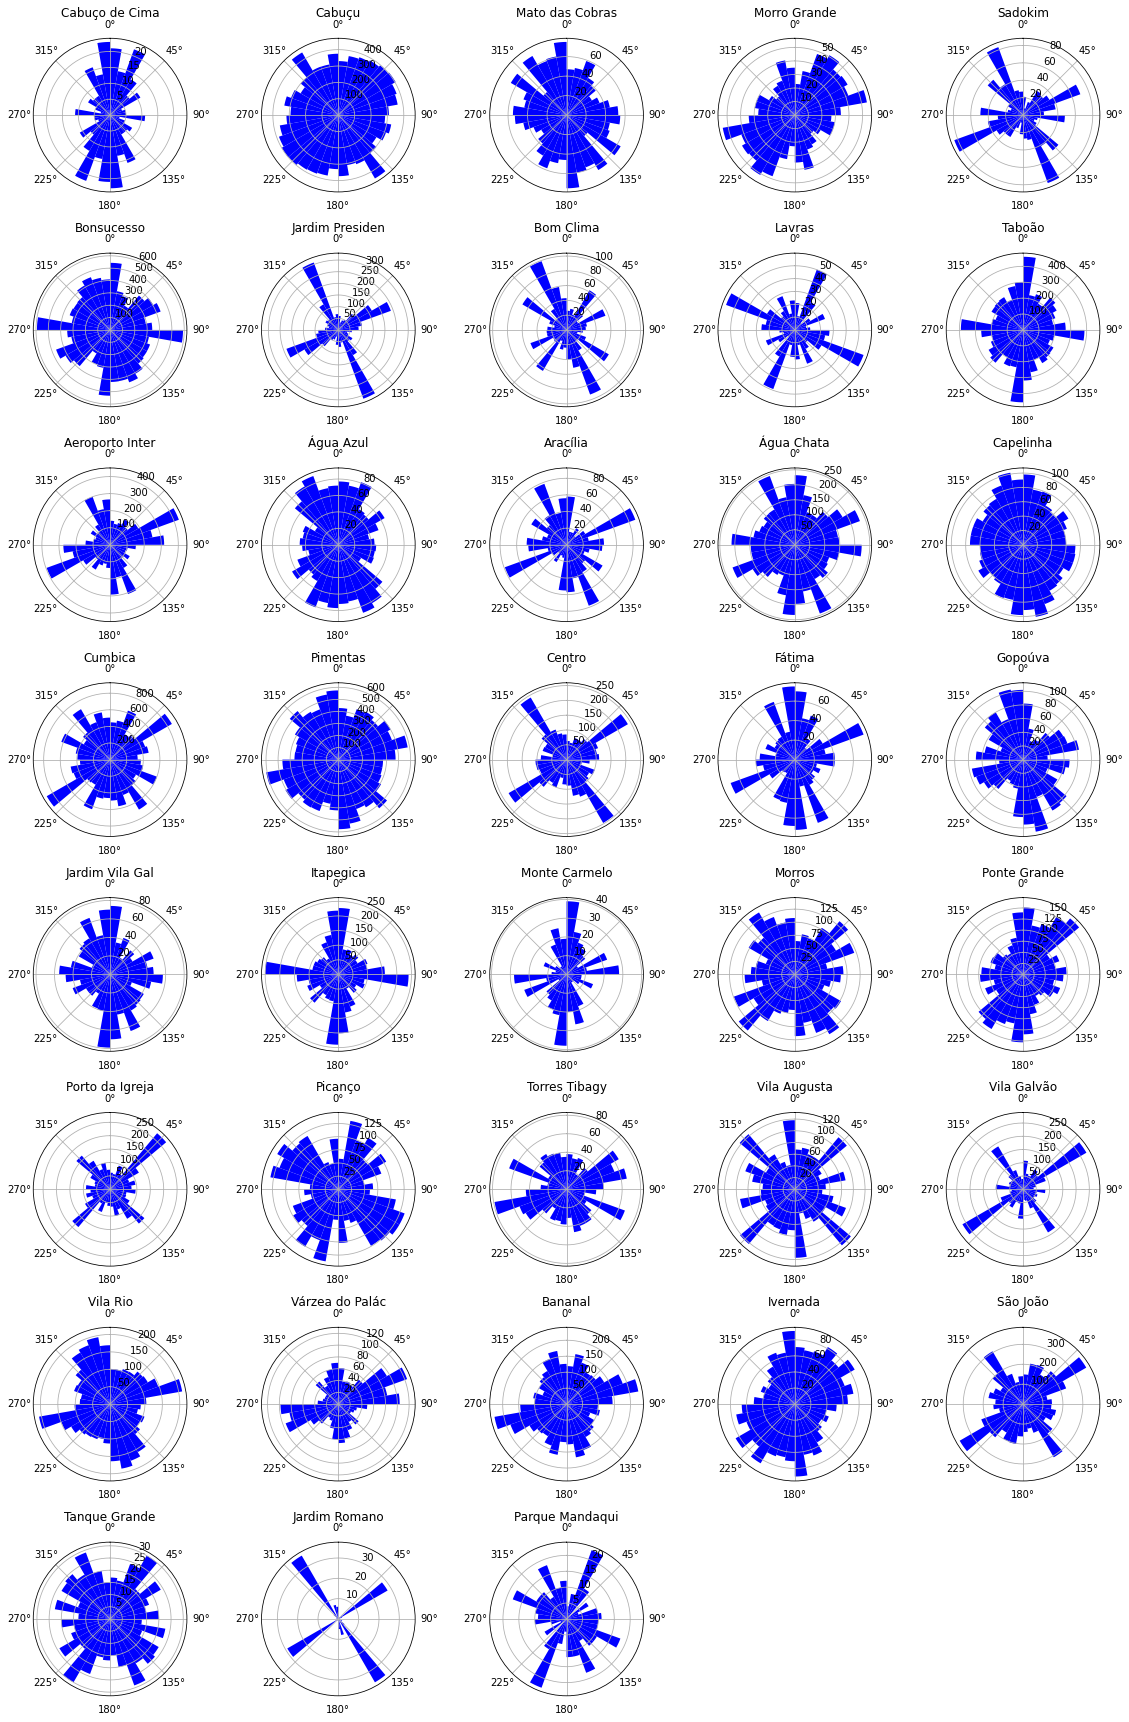
\includegraphics[width=.9\textwidth]{images/8_appendix/polar_plots_guarulhos.png}
    \caption*{\ Fonte: Produzido pelos autores Fernandes \& Alves}
    \label{fig:bearing_bairros}
\end{figure}


\section{Demais cidades}

Para visualizar os resultados relativos às outras cidades, é possível acessar o seguinte endereço: \url{https://github.com/Gui-FernandesBR/Last-Mile-Routing-Analyzer/tree/master/results}.
